\section{Model mismatch: Gaussian Process}

In case of model mismatch, i.e., when the observed data is not distributed according
a Gaussian Markov Random Field (GMRF) with a Laplacian matrix as its precision matrix,
then our method estimates the closest graph Laplacian fit with respect to the original
model, as done similarly by GGL (see Egilmez \textit{et. al.} 2017).

In this section, we show results from experiments in which the underlying covariance
matrix is modeled as two-dimensional functions that often appear in the literature of
Gaussian process regression.

We consider that the data $\bm{Y}$ is distributed according to a multivariate Gaussian with
zero mean vector and covariance matrix
$[\boldsymbol{\Sigma}]_{ij} = \sigma_1 \exp{\left(-l_1 \sin^2\left(\frac{\pi|\bm{x}_i - \bm{x}_j|}{p}\right)\right)}
+ \sigma_2 \exp{\left(-l_2|\bm{x}_i - \bm{x}_j|^2\right)}$.

\begin{figure}[!htb]
    \centering
    \begin{subfigure}[b]{0.3\textwidth}
      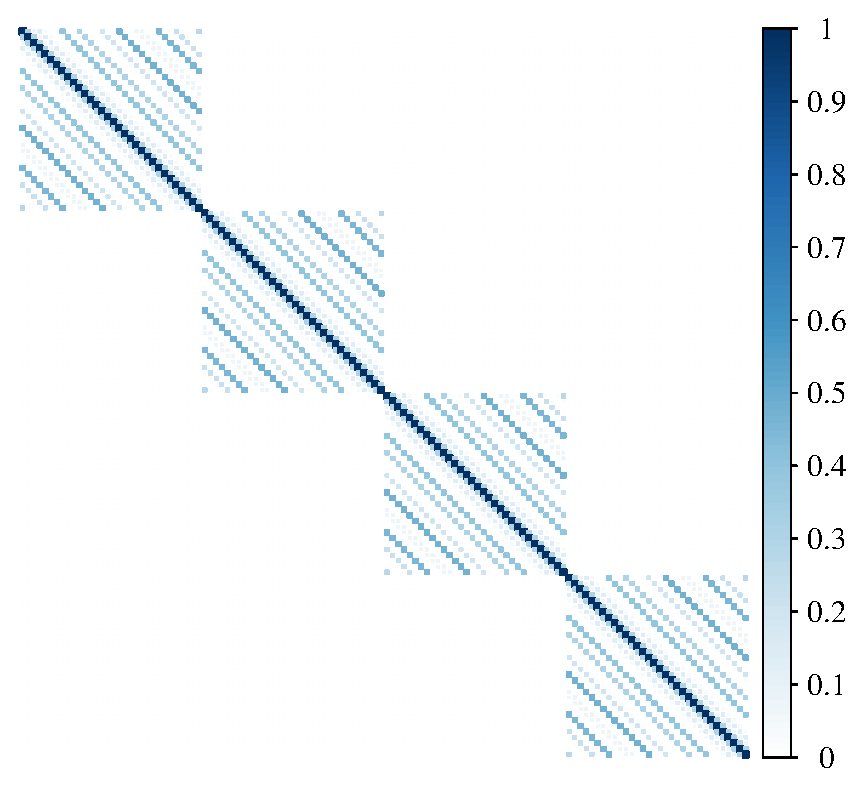
\includegraphics[width=\textwidth]{gaussian-process/latex/figures/periodic_gaussian_block_covariance.eps}
        \caption{Ground Truth Covariance}
    \end{subfigure}
    \hfill %add desired spacing between images, e. g. ~, \quad, \qquad, \hfill etc.
      %(or a blank line to force the subfigure onto a new line)
    \begin{subfigure}[b]{0.3\textwidth}
        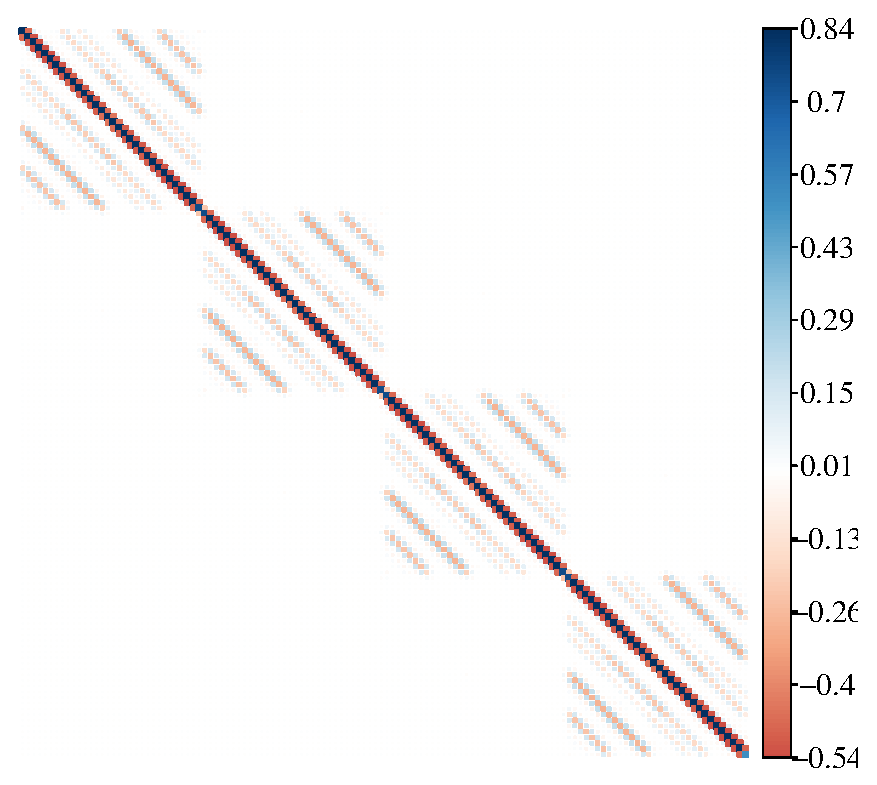
\includegraphics[width=\textwidth]{gaussian-process/latex/figures/periodic_gaussian_block_precision.eps}
        \caption{Ground Truth Precision}
    \end{subfigure}
    \hfill %add desired spacing between images, e. g. ~, \quad, \qquad, \hfill etc.
    %(or a blank line to force the subfigure onto a new line)
    \begin{subfigure}[b]{0.3\textwidth}
        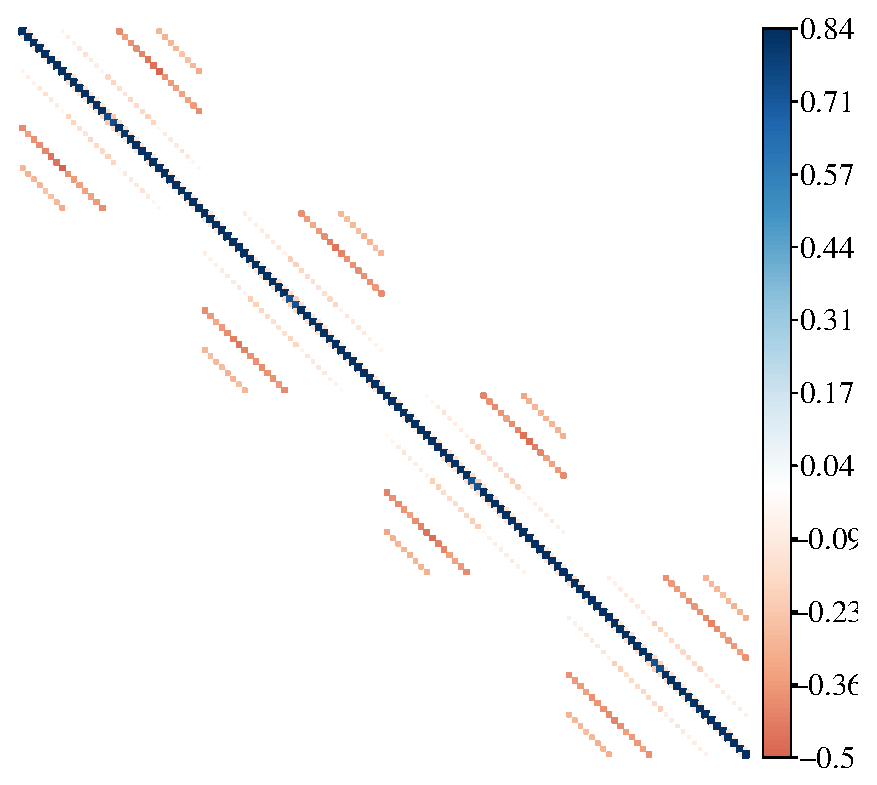
\includegraphics[width=\textwidth]{gaussian-process/latex/figures/periodic_gaussian_block_laplacian.eps}
        \caption{Learned Laplacian}
    \end{subfigure}
    \caption{add caption}
        \label{fig:gps}
\end{figure}
